\subsection{Modellierung der Systemdynamik}
In diesem Abschnitt werden die Bewegungsgleichungen des 3D-Modells mit Hilfe des Lagrange-Formalismus hergeleitet. Der Würfelkörper besitzt drei rotatorische Freiheitsgrade, die drei Schwungmassen verfügen über jeweils einen Freiheitsgrad. Somit ergeben sich insgesamt sechs Freiheitsgrade für das Gesamtsystem. Dadurch steigt die Komplexität der Systemdynamik stark an, allerdings bestehen nach wie vor Parallelen zu der Dynamik des 1D-Modells.
\newline

Um die Position des Würfels zu beschreiben wird ein raumfestes Bezugssystem $\{I\}$ eingeführt, welches von den drei Einheitsvektoren $\inI e_x$, $\inI e_y$ und $\inI e_z$ beschrieben wird. Das zweite Bezugssystem $\{W\}$ ist körperfest und rotiert somit mit dem Würfel. Es wird von den Einheitsvektoren $\inW e_x$, $\inW e_y$ und $\inW e_z$ beschrieben.

\begin{figure}[h]
\centering
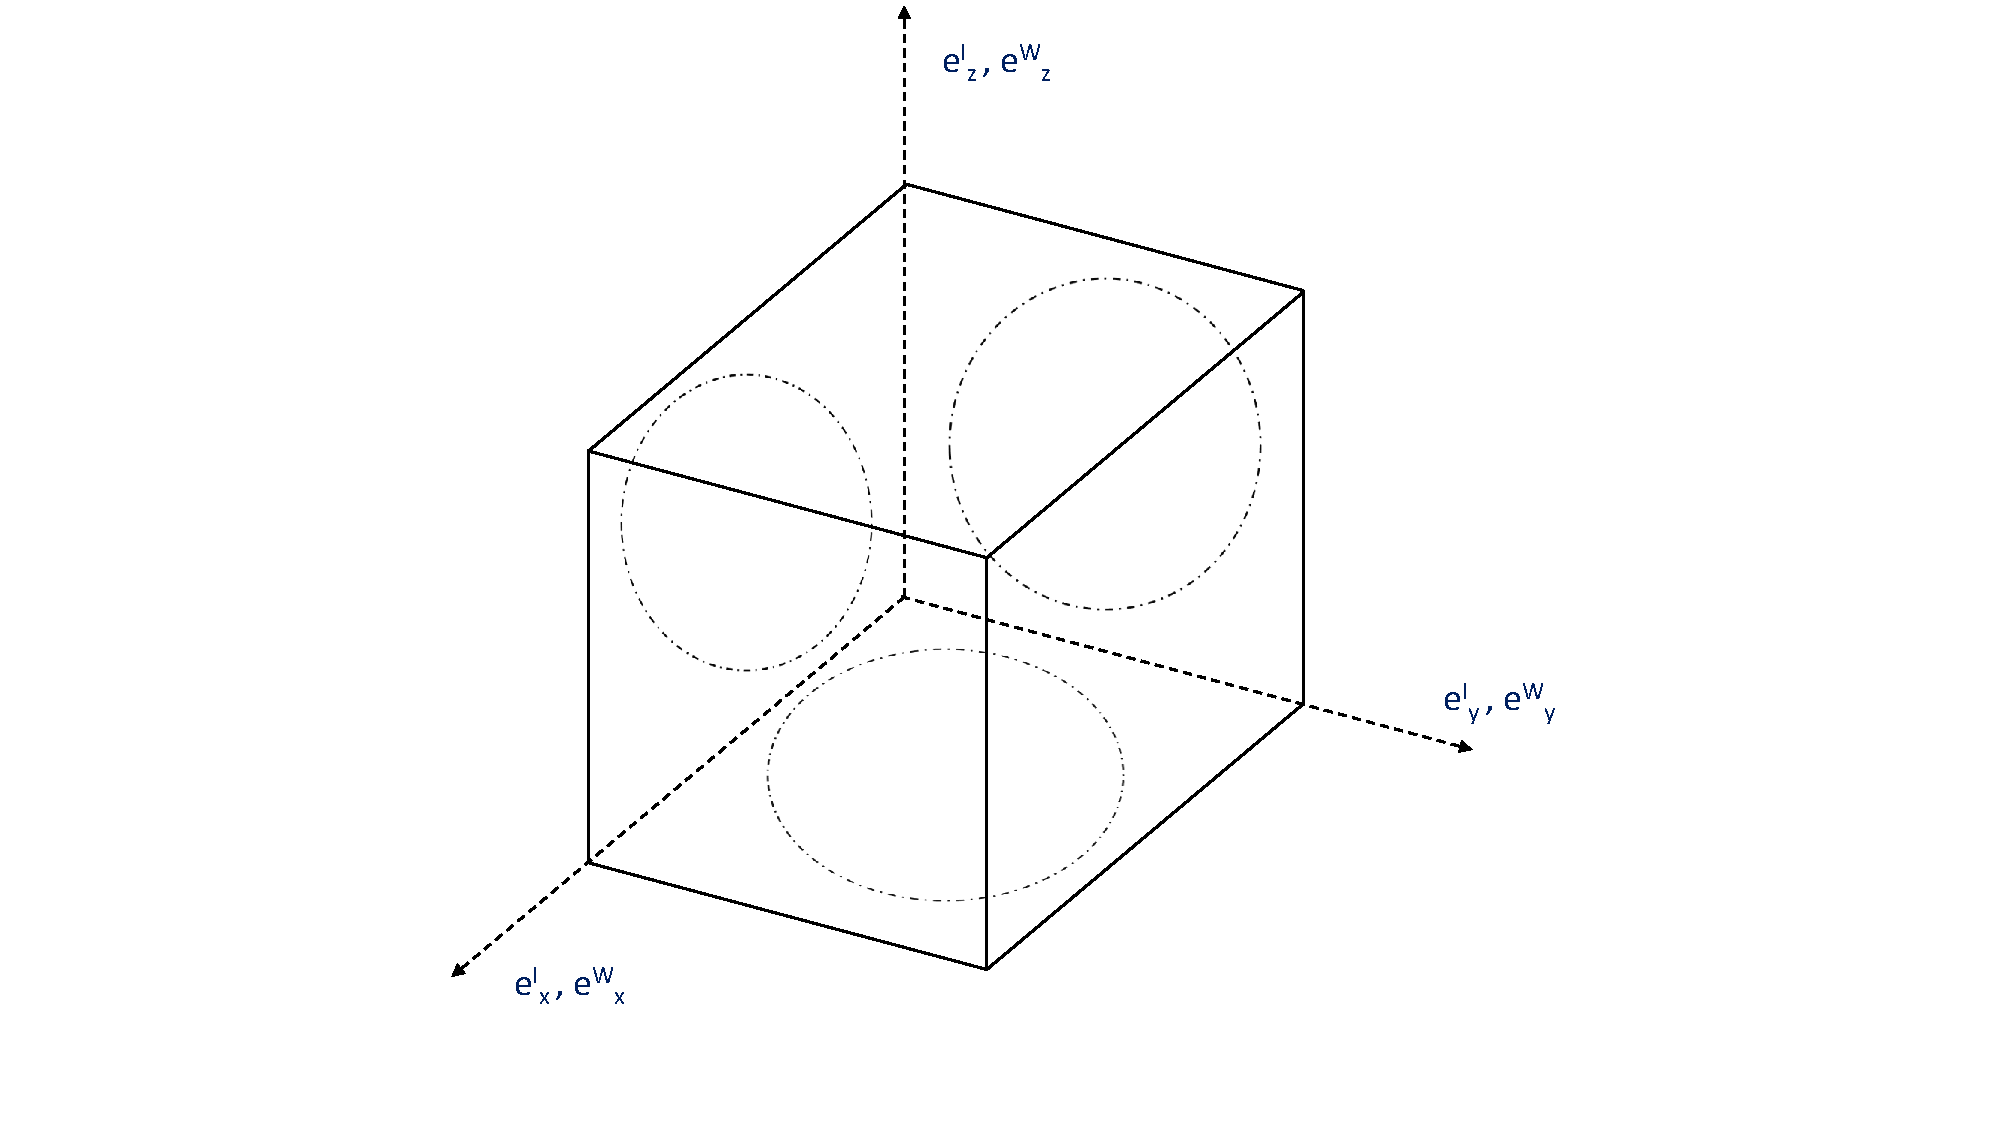
\includegraphics[width=\linewidth]{MechZeichnung3D}
\caption{Mechanischer Aufbau, Quelle: eigene Darstellung}
\end{figure}

Die aktuelle Position des Würfels kann somit eindeutig durch die Verschiebung des körperfesten Bezugssystems $\{W\}$ zu dem raumfesten Bezugssystem $\{I\}$ bestimmt werden. Um diese Rotation zu beschreiben werden die drei Euler-Winkel $\varphi_1$, $\varphi_2$ und $\varphi_3$ eingeführt. Die Drehreihenfolge und Drehachsen werden im folgenden beschrieben.

\begin{table}[h]
\centering
\begin{tabular}{|c|c|}
\hline
\textbf{Winkel} & \textbf{Beschreibung} \\ \hline
$\varphi_1$ & Drehung um $\inI e_z$ \\ \hline
$\varphi_2$ & Drehung um $\inW e_x$  \\ \hline
$\varphi_3$ & Drehung um $\inW e_z$ \\ \hline
\end{tabular}
\end{table}

Mit Hilfe der Euler-Winkel können Drehmatrizen definiert werden um Koordinaten in dem raumfesten Bezugssystem $\{I\}$ in das körperfeste Bezugssystem $\{W\}$ zu projizieren. Hier zeigt sich wieder die Bedeutung der Reihenfolge der einzelnen Drehungen, da auch die Matrizenmultiplikation im Allgemeinen nicht kommutativ ist.

\begin{equation}
\inW{}\boldsymbol{r} = \inW{}\bS{D}_{\varphi_1} \cdot \inW{}\bS{D}_{\varphi_2} \cdot \inW{}\bS{D}_{\varphi_3} \cdot \inI{}\bS{r} = \inW{}\bS{D} \cdot \BinI{r}
\end{equation}
\begin{equation}
\inW{}\bS{D}_{\varphi_1} = \begin{pmatrix}
c_{\varphi_1} & -s_{\varphi_1} & 0 \\
s_{\varphi_1} & c_{\varphi_1} & 0 \\
0 & 0 & 1
\end{pmatrix}
\hspace{5pt}
\inW{}\bS{D}_{\varphi_2} = \begin{pmatrix}
1 & 0 & 0 \\
0 & c_{\varphi_2} & -s_{\varphi_2} \\
0 & s_{\varphi_2} & c_{\varphi_2}
\end{pmatrix}
\hspace{5pt}
\inW{}\bS{D}_{\varphi_3} = \begin{pmatrix}
c_{\varphi_3} & -s_{\varphi_3} & 0  \\
s_{\varphi_3} & c_{\varphi_3} & 0 \\
0 & 0 & 1
\end{pmatrix}
\end{equation}
\begin{equation}
\BinW{D} = \begin{pmatrix}
c_{\varphi_1}c{\varphi_3} - s_{\varphi_1}c_{\varphi_2}s_{\varphi_3} &
-c_{\varphi_1}s_{\varphi_3} - s_{\varphi_1}c_{\varphi_2}c_{\varphi_3} &
s_{\varphi_1}s_{\varphi_2} \\
s_{\varphi_1}c_{\varphi_3}+c_{\varphi_1}c_{\varphi_2}s_{\varphi_3} &
-s_{\varphi_1}s_{\varphi_3}+c_{\varphi_1}c_{\varphi_2}{\varphi_3} &
-c_{\varphi_1}s_{\varphi_2} \\
s_{\varphi_2}s_{\varphi_3} &
s_{\varphi_2}c_{\varphi_3} &
c_{\varphi_2}
\end{pmatrix}
\end{equation}

Die Projizierung einer Koordinate aus dem körperfesten in das raumfeste Bezugssystem erfolgt durch die transponierte der Matrix $\BinW{D}$.

\begin{equation}
\BinI{r} = \BinI{D} \cdot \BinI{r} = \BinW{D}^T \cdot  \BinI{r}
\end{equation} 

Die Bewegung der Schwungmassen relativ zu dem Würfelkörper wird von den drei Winkeln $\psi_1$, $\psi_2$ und $\psi_3$ beschrieben. Deren zeitliche Ableitungen stellen die Winkelgeschwindigkeiten der Schwungräder dar. 

\begin{equation}
\bS{\psi} = \begin{pmatrix}
{\psi}_1 \\
{\psi}_2  \\
{\psi}_3 
\end{pmatrix}
\hspace{35pt}
\bS{\dot{\psi}} = \begin{pmatrix}
\dot{\psi}_1 \\
\dot{\psi}_2  \\
\dot{\psi}_3 
\end{pmatrix}
\end{equation}

\subsubsection{Potential des Systems}
Um die Lagrange-Funktion $L$ des Systems zu bestimmen muss einerseits die kinetische Energie $T$ und die potentielle Energie $V$ ermittelt werden. Das Potential des Würfels wird durch die aktuelle Lage seines Schwerpunktes $\bS{r}$ bestimmt, hierbei ist lediglich die z-Komponente des raumfesten Bezugssystem von Bedeutung.

\begin{equation}
V = m_G \cdot g \cdot \inI z_{cog}
\end{equation}

Die Position des Schwerpunktes im körperfesten Bezugssystem ist fix. Durch die Projektion dieses Vektors $\BinW{r}_{cog}$ in das raumfeste Bezugssystem $\{I\}$ wird die Abhängigkeit von der aktuellen Verschiebung berücksichtigt.

\begin{equation}
\BinI{r}_C = \BinI{D} \cdot \BinW{r}_{C} = \BinI{D} \cdot \begin{pmatrix}
\inW x_C \\ \inW y_C \\ \inW z_C
\end{pmatrix}
\end{equation}

Folglich ergibt sich der folgende Zusammenhang für das Potential $V$ und die aktuelle Ausrichtung des Würfels.

\begin{equation}
V = m_G \cdot g \cdot \inI z_{cog} = m_G \cdot g \cdot (s_{\varphi_2}s_{\varphi3} \cdot \inW x_C + s_{\varphi_2}c_{\varphi_3} \cdot \inW y_C  + c_{\varphi_2} \cdot \inW z_C)
\end{equation}

\subsubsection{Kinetische Energie des Systems}
Die kinetische Energie setzt sich aus der Winkelgeschwindigkeit des Würfels $\bS{\omega}_K$ und der Geschwindigkeiten der drei Schwungmassen $\bS{\omega}_R$ zusammen. Hierbei ist zu beachten, dass die Winkelgeschwindigkeiten in verschiedenen Bezugssystemen darstellbar sind und die kinetische Energie von der Darstellungsform unabhängig ist. Um dies zu gewährleisten müssen allerdings auch die Trägheitstensoren in das jeweilige Bezugssystem projiziert werden.

\begin{equation}
\BinW{\omega}_K = \begin{pmatrix}
\inW \omega_x \\
\inW \omega_y \\
\inW \omega_z
\end{pmatrix}
\hspace{35pt}
\BinW{\omega}_R = \dot{\bS{\psi}}
\end{equation}

\begin{equation}
T = \frac{1}{2} \BinW{\omega}^T_K \cdot (\BinW{\Theta}_G - \BinW{\Theta}_R) \cdot \BinW{\omega}_K + \frac{1}{2} (\BinW{\omega}_K + \BinW{\omega}_R)^T \cdot \BinW{\Theta}_R \cdot (\BinW{\omega}_K + \BinW{\omega}_R)
\end{equation}

\subsubsection{Generalisierte Kraftkomponenten}
In der Untersuchung des 1D-Modelles wurde bereits gezeigt, dass der Würfel ein nicht konservatives System ist, da einerseits über die Motoren mechanische Energie zugeführt wird und andererseits durch Reibung mechanische Energie verloren geht. Deshalb müssen die generalisierten Kraftkomponenten bestimmt werden um mit Hilfe des d'Alembert'schen Prinzip die Bewegungsgleichungen zu ermitteln.
\newline

Wie bereits angesprochen erzeugen die Motoren Momente, welche die Schwungmassen antreiben. Gleichermaßen entsteht in den Lagern der Räder ein Reibmoment welches als linear abhängig von der Winkelgeschwindigkeit modelliert wird. Somit ergibt sich das folgende Moment.

\begin{equation}
\BinW{M}_M = \BinW{T}_M - \bS{C}_{\psi} \cdot \BinW{\dot {\psi}} \hspace{35pt} \bS{C}_{\psi} = \begin{pmatrix}
C_{\psi_1} & 0 & 0 \\
0 & C_{\psi_2} & 0 \\
0 & 0 & C_{\psi_3}
\end{pmatrix}
\end{equation}

Das von der Gravitation verursachte Moment $M_G$ lässt sich aus der aktuellen Position des Schwerpunktes $\bS{r}_C$ und der Schwerkraftvektors $\bS{g}$ berechnen.

\begin{equation}
\BinI{G} = \begin{pmatrix}
0 \\ 0 \\ -m_G \cdot g
\end{pmatrix}
\hspace{35pt}
\BinW{G} = \BinW{D} \cdot \BinI{G} = -m_G \cdot g \cdot \begin{pmatrix}
s_{\varphi_1}s_{\varphi_2} \\ -c_{\varphi_1}s_{\varphi_2} \\ c_{\varphi_2}
\end{pmatrix}
\end{equation}

\begin{equation}
\BinW{M}_G = \BinW{r}_C \times \BinW{G} = -m_G \cdot g \cdot  \begin{pmatrix}
\inW y_C \cdot c_{\varphi_2} + \inW z_c \cdot c_{\varphi_1} s_{\varphi_2} \\
\inW z_C \cdot s_{\varphi_1}s_{\varphi_2} - \inW x_C \cdot c_{\varphi_2} \\
- \inW x_C \cdot c_{\varphi_1}s_{\varphi_2} - \inW y_C \cdot s_{\varphi_1} s_{\varphi_2} 
\end{pmatrix} 
\end{equation}